% --------------------------------------------
%		CAPITOLO 3 
%---------------------------------------------
\chapter{VTX detector}

This chapter focuses on one of the four proposal for the vertex detector upgrade of Belle II, that is VTX. After a brief reference to the reasons behind the vertex detector upgrade, we will go trough VTX concept and layout, designed with a new geometry with respect VXD and so with a different mechanical structure and a new pixel sensor, in order to fullfil the new requirements dictated by new environment conditions. Moreover all ongoing studies are supported by continual tests and simulations that we will also take a look at.


%---------------------------------------------
%			3.1
%---------------------------------------------
\section{VTX Layout and mechanical structure?}

In section \vpageref{nano_beam} we have introduced in a few word the concept of the \textit{nano-beam} scheme, which could allow to achieve the new fixed target of istantaneous luminosity. This new strategy required a strong focusing of the beams in particular at the IP, resulting in a large amounts of beam induced background and as consequence in a higher dose of radiation in the innermost detector layers, which therefore have to be robust enough to keep good performance.
Furthermore, to be able to reach the target luminosity, SuperKEKB might have to consider an improvements of the final focusing magnets and so a potentially re-design of the interaction region, including the detector (regardless of the hit rates and radiation hardness issue?).\\

\begin{figure}[h!]
\centering
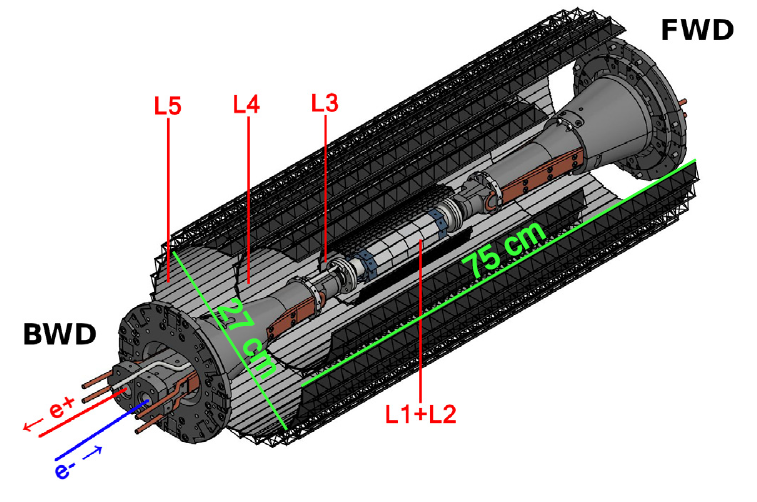
\includegraphics[scale=.6]{VTX_layers}
\caption{Concept of VTX layout with 5 barrel layers, filling the current VXD volume.}
\label{fig:VTX_layers}
\end{figure}


So VTX aims to replace the all VXD with a fully pixelated detector based on Depleted Monolithic Active Pixel Sensors (DMPAS) arranged on five layers at different distance from the beam pipe. Acutally the radii and the number of the layers are currently subject to studies and simulations in order to achieve an optimized arrangement(?) (figure \vpageref{fig:VTX_layers}). 
As already discussed for other upgrade proposal, it may be important to try to reduce the material budget, in order to minimize the multiple Coulomb scattering which particularly affects the very soft particles produced in Belle II collisions. By using a single sensor type, it is expected a reduction of the overall material budget up to 2\% of radiation lenght, against the present 3\% of VXD, which uses two different sensors such as pixels and strips.


\subsection{iVTX}

The \textit{internal}VTX consists of the first two detector layers devised togheter with a self-supported air-cooled all-silicon ladder concept, where four contiguous sensors are diced out of a wafer, thinned and interconnected with post-processed redistribution layers. They are designed to be at 1.4 and 2.2 cm respectively from the beam pipe, and to target an individual material budget of about 0.1\% radiation lenght. This is actually achivable because the overall surface of this layers is moderate, below 400 $cm^{2}$, the low sensor power dissipation and the few connections needed for the operation.  

%eye ??


\begin{figure}[h!]
\centering
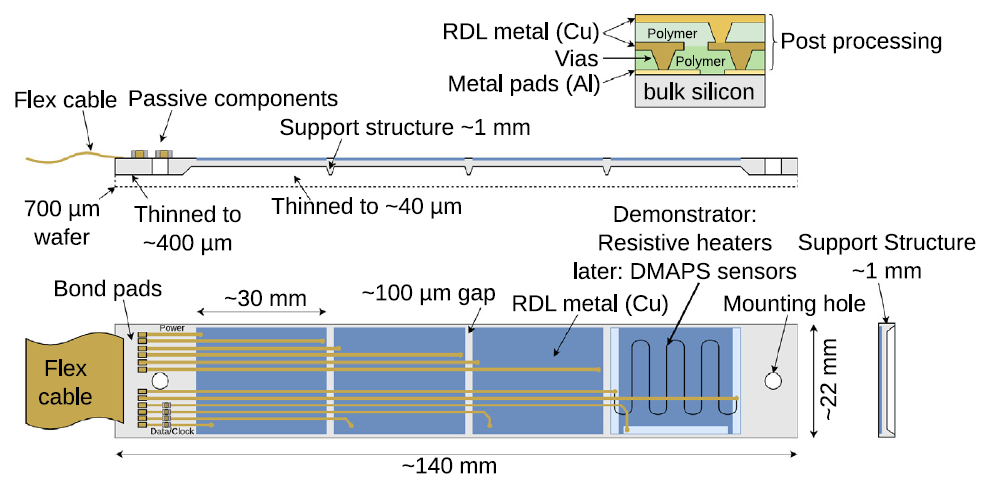
\includegraphics[scale=.65]{iVTX}
\caption{Sketch of the all-silicon ladder concept of the iVTX. Four dummy sensors are shown in blue on the silicon support in grey. The yellowish lines instead, indicate power and data transmission lines. Power is delivered to the ladder by a flex cable, which also transmits data to and from the chips in the final chips.}
\label{fig:iVTX}
\end{figure}

In figure \vpageref{fig:iVTX} is showing a sketch of the iVTX demonstrator ladder, 140 mm long and 22 mm wide (grey). Instead of the actual sensors, it is equipped with four dummies chips with a lenght of about 30 mm (blue), which are used as resistor to mimic the estimated heat load in order to test the air cooling system. A redistribution layers (RDL) for power and data is also added to the demonstrator, to connect the chips with a flex cable at the end of the ladder (yellowish lines). In addition the wafer is thinned to 400 $\mu$m and the sensitive areas down to 40 $\mu$m, to test the mechanical integrity.

\subsubsection{R\&D}

The R\&D in ongoing. First thinned ladders have been produced and characterised with different thickness and geometry, revealing a homogeneous thickness over an area of 10 $cm^{2}$. 

In addition tests are focused on evaluating power delivery efficiency, the quality of the signal which travel through the ladder and also the process used to fully assembly it. 
In figure \vpageref{fig:iVTX_eye} are shown eye diagrams from simulation with a transfer rate of 640 Mbps, which may imply that 320 Mbps of data rate will be possible. (??) 

\begin{figure}[h!]
\centering
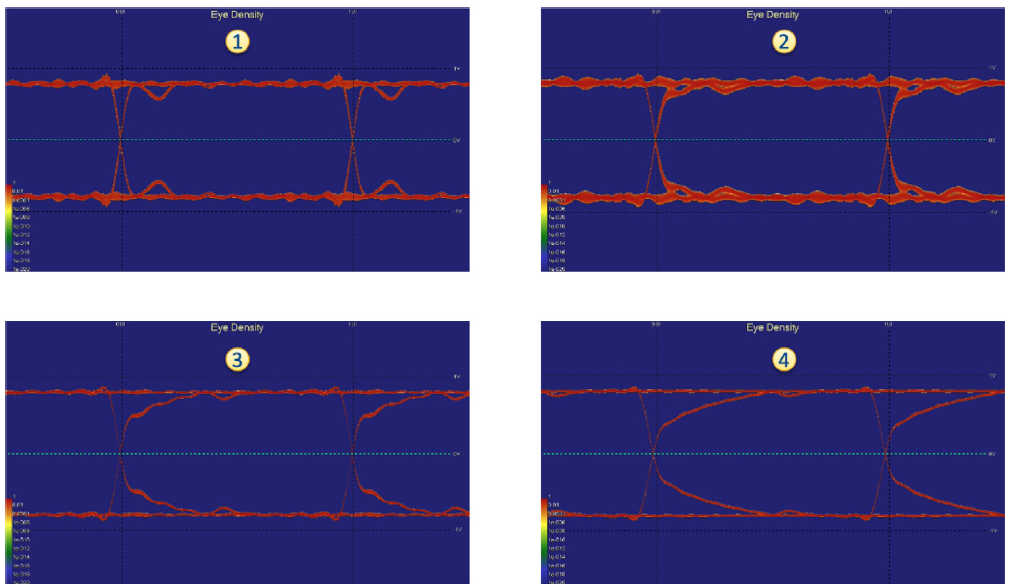
\includegraphics[scale=.7]{iVTX_eye}
\caption{Eye diagrams of the iVTX data transmission lines at four different locations on the ladder.}
\label{fig:iVTX_eye}
\end{figure}


\subsection{oVTX}

The \textit{outer?}VTX consists of three layers respectively at radii of 3.9, 9 and 14 cm from the beam pipe and because of the larger distance required to cover the acceptance, they are not self-support. They follow a more traditional approach, strongly inspired by the designed developed for the ALICE ITS2. Each ladder is water cooled and made of a light carbon fiber support structure, called \textit{truss}, which provide the mechanical integrity. Its structural design is showed in figure \vpageref{fig:oVTX}: 70 cm long and 5.8 g of weight, it is able to support more than 40 sensors in two rows next to each other with a small overlap, earning a material budget of 0.3\% $X_{0}$ for the first two layer and 0.8\%$X_{0}$  for the outermost one.

\begin{figure}[h!]
\centering
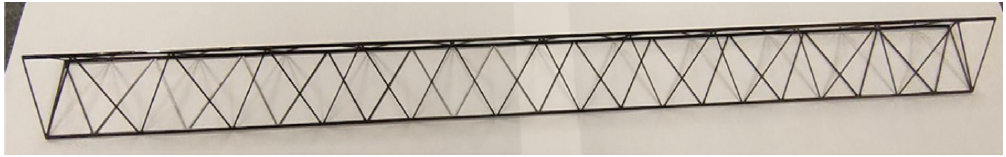
\includegraphics[scale=.7]{oVTX}
\caption{Prototype of the layer 5 \textit{truss}, which is the longest, made from thin carbon fibre structures.}
\label{fig:oVTX}
\end{figure}


For the cooling of the ladder, it is developing a cold-plate concept (figure \vpageref{oVTX_coldplate}), on which the sensors are glued and that in turn is installed on the truss. For each row, there is a polymide cooling tube that runs over all the sensors and turns back at the other end, so that the heated coolant leaves on the same side.

\begin{figure}[h!]
\centering
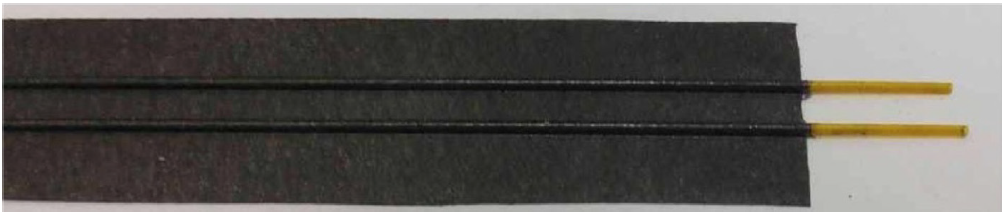
\includegraphics[scale=.7]{coldplate}
\caption{A prototype of the cold-plate for colling. One coolant tube(golden) is connected to the cold plate(black) and turns 180° on the other end (not shown) so that the coolant flows in both directions and thus leaves on the same side it starts.}
\label{fig:oVTX_coldplate}
\end{figure}


In figure \vpageref{fig:oVTX_5} is shown the several structures described that shape a ladder of the outermost layer 5. From bottom to top come in succession the carbon fibre structure, two cold-plates for the two neighbouring sensor rows (Chips, in grey) and the flex cables for power and data transmission (green). 


\begin{figure}[h!]
\centering
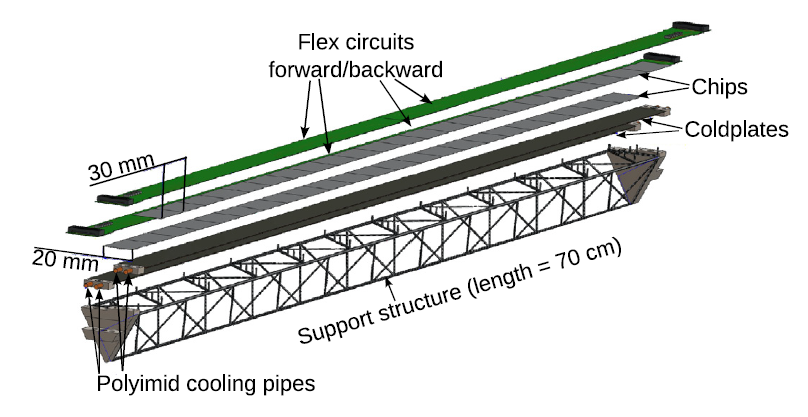
\includegraphics[scale=.7]{oVTX_5}
\caption{An exploding drawing of a fully assembled layer 5 ladder.}
\label{fig:oVTX_5}
\end{figure}

\subsubsection{R\&D}

After the assembly described in the previous, first thermo-mechanical tests were performed and they show that the first resonance frequency is at 200 Hz, which is above the one of the typical earthquakes in Japan and also that the thermal properties are good.\\

Trying to reduce as much as possible the material budget, the transmission lines and the flex cables has to be as thin as possible, but also need to ensure safe data transmission. For this reason, the outermost ladders long 70 cm are equipped with two flex cables, one from each side of the \textit{truss}. In figure \vpageref{fig:oVTX_eye} the resulting eye diagram from testing the signal integrity of one of the 35 cm long transmission lines for data transmission rate of 500 Mbps. A clear difference between high and low indicates a good starting point for further developments. 


\begin{figure}[h!]
\centering
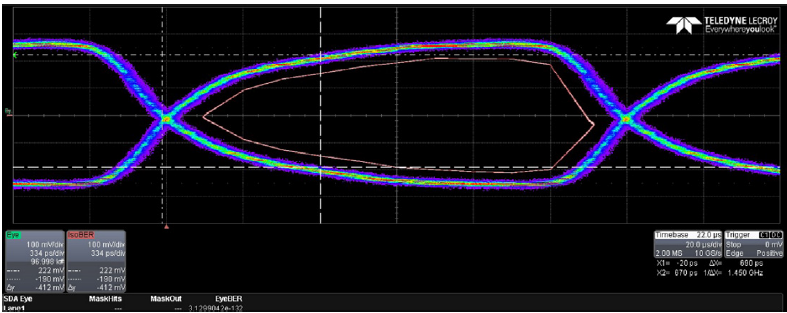
\includegraphics[scale=.8]{oVTX_eye}
\caption{Eye diagram for the oVTX transmission line signal integrity of the layer 5 flex cable.}
\label{fig:oVTX_eye}
\end{figure}


%---------------------------------------------
%			3.2
%---------------------------------------------
\section{Performance simulation}
%richiesta sensitivity di 150 um ? VTX article, betagamma


%---------------------------------------------
%			3.3
%---------------------------------------------
\section{OBELIX chip design}

As we already seen, the VTX detector is designed with a single type sensor taylored to the specific need of Belle II, called OBELIX (Optimized BELle II pIXel sensor) and currently under development, based on fast and high granular Depleted Monolithic Active Pixel Sensor (DMAPS). This new designed sensor comes from an evolution of TJ-Monopix 2, whose characterization is the main topic of this thesis, and which will be discussed in (reference) and both of them relie on the CIS? 180 $\mu$m process by TowerJazz Semiconductor.
As a matter of fact its predecessor is equipped with four different flavors (reference), and for now the final decision on which to use for Obelix has not been made. \\

\begin{figure}[h!]
\centering
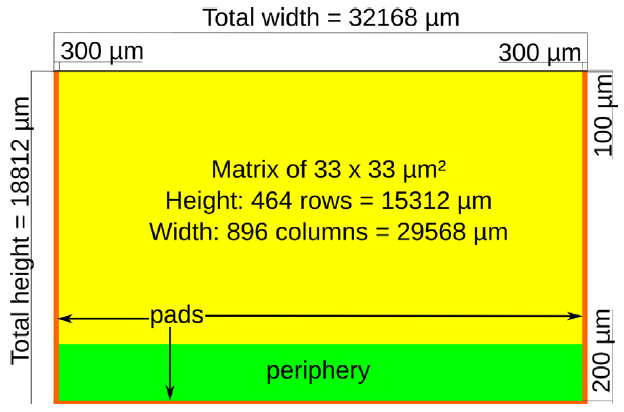
\includegraphics[scale=.7]{obelix_schematic}
\caption{OBELIX chip design.}
\label{fig:obelix_scheme}
\end{figure}

A schematic  layout of the chip is shown in figure \vpageref{fig:obelix_features}. The size of the sensor is expected to be 3 x 2 $cm^{2}$, with an active area of 3 x 1.5 $cm^{2}$ and an additional part in the periphery of about 3 x 0.3 $cm^{2}$ dedicated to data pre-processing and triggering. The pixel pitches are designed to be from 30 $\mu$m to 40 $\mu$m in both direction. 
To deal with the target hit rate of 120 MHz/$cm^{2}$, the timestamp clock signal can reach down to 25 ns, even if studies have demonstrated that a window of 100 ns is enough to limit to 320 Mbps the data throughput at the same expected hit rate.
With respect to TJ-Monopix 2, which is equipped with a triggerless column-drain readout without memory at the periphery, OBELIX must have a triggered readout architecture, in order to satisfy the needs of Belle II. Moreover the latency is fixed to 5 $\mu$s and it might operate up to 30 KHz trigger rate.
The expected power consumption instead, is expected to be about 200 mW/$cm^{2}$. 

Its main design features are summarised in \vpageref{fig:obelix_scheme}.


\begin{figure}[h!]
\centering
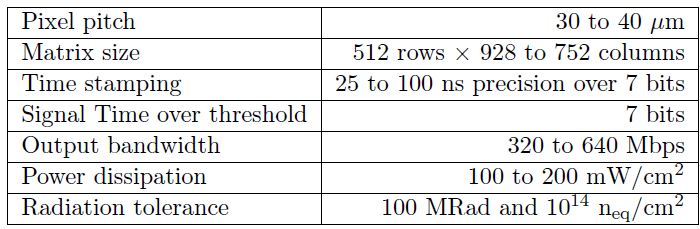
\includegraphics[scale=.7]{obelix_features}
\caption{Designed features of the OBELIX sensor.}
\label{fig:obelix_features}
\end{figure}





\begin{comment}
%---------------------------------------------
%			3.4
%---------------------------------------------
\section{Mechanical structure}

%% Struttura Layer
%% Sistema di cooling 
%% Connessioni?

\end{comment}




%---------------------------------------------
%		BIBLIOGRAFIA
%---------------------------------------------

%TVX ARTICLE
%CDR
%LUDO
%VTX proposal


%---------------------------------------------
%		COMMENT
%---------------------------------------------
